\documentclass[11pt]{article}

% --- Packages ---
\usepackage[margin=0.7in]{geometry}
\usepackage{amsmath,amssymb}
\usepackage{graphicx}
\usepackage{float}
\usepackage{booktabs}
\usepackage{hyperref}
\usepackage{setspace}
\usepackage{caption}
\usepackage{subcaption}
\usepackage{xcolor, soul}
\usepackage{colortbl}

% --- Setup hyperref ---
\hypersetup{
    colorlinks=true,
    linkcolor=blue,
    filecolor=magenta,
    urlcolor=cyan,
    citecolor=blue,
}

% --- Title Information ---

\title{\textbf{Final Project Report:\\How Music Taste Changes Over Time}}

\author{
    Lauren Yee, 
    Kian Sharifzadeh, 
    Krish Doshi \\
    \vspace{0.3cm}
    \textit{STAT 423: Applied Linear Regression $\&$ ANOVA}
}
\date{\today}

\begin{document}

\maketitle

\begin{abstract}
Music is a key part of daily life, yet musical preferences evolve over time. 
This study examines how various song and artist characteristics influence ratings of Billboard Hot 100 Number One songs. 
Data from the 1960s through the 2010s were grouped by decade. Before stepwise selection using AIC, the main effects model and model including interaction terms were compared.
Comparing the optimized models for each decade revealed that the predictors of song ratings vary over time, with no single factor remaining consistently significant across all decades.
\end{abstract}

\onehalfspacing
 
{\scriptsize First author: Krish}
% -------------------------------------------------------------------
\section{Introduction}
% -------------------------------------------------------------------

\textbf{\underline{Research Questions}}

\begin{enumerate}
\item What are the most and least optimal predictors over time from 1960--2010?
\item How do the models stay consistent and how do they change?
\item How does the predictive power of predictors change over time and which model performs best?
\end{enumerate}

Our interest in music inspired our group to investigate how musical preferences change through time. 
Different characteristics of songs and artists may influence how highly a song is rated.
By comparing these predictors across time periods, this study highlights how trends and artist characteristics relate to song ratings.

{\scriptsize First author: Kian}
% -------------------------------------------------------------------
\section{Data Description and Exploratory Data Analysis (EDA)}
% -------------------------------------------------------------------

This dataset includes information about every Number 1 song on the Billboard charts from 1958--2025. It was compiled
by Chris Dalla Riva (singer, songwriter, and data expert), who listened to each number one hit song and tracked data related to each song.
Most of the data comes from facts about the song, Chris's interpretation of the song, or data and ratings from Spotify.
Upon data cleaning, we found missing values among the predictors used in the models, reducing the size of the dataset from 1177 rows to 1154 rows. 
Missing values occurred in different single-digit counts and were not concentrated in earlier decades such as the 1960s, implying that the missingness was unsystematic.

{\scriptsize First author: Krish}

\subsection{Variables}
Let $Y$ denote the overall rating of the song. Our predictors are:

\begin{itemize} 
\item $X_1$: Age: Average age of the artist(s) 
\item $X_2$: GenderNotMale: Whether any of the artists aren't male (1 if not male, 0 otherwise) 
\item $X_3$: RaceWhite: If any of the artists are white (1 if white, 0 otherwise) 
\item $X_4$: GenreJazz: If the song is jazz (1 if jazz, 0 otherwise) 
\item $X_5$: GenreRock: If the song is rock (1 if rock, 0 otherwise) 
\item $X_6$: GenrePop: If the song is pop (1 if pop, 0 otherwise) 
\item $X_7$: GenreOther: If the song genre isn't specified (1 if not specified by other variables and 0 otherwise) 
\item $X_8$: Energy: Energy measure from Spotify (0-100) 
\item $X_9$: Danceability: Danceability measure from Spotify (0-100) 
\item $X_{10}$: Happiness: Happiness measure from Spotify (0-100) 
\item $X_{11}$: Loudness\_db: Loudness measured in decibels from Spotify 
\item $X_{12}$: BPM: Beats per minute from Spotify 
\item $X_{13}$: Length\_sec: Length of the song in seconds 
\end{itemize}

{\scriptsize First author: Kian}


\subsection{Exploratory Analysis}
\noindent To narrow our scope, we focused on song characteristics and artist's traits. 
First, we look at the numeric predictors: energy, danceability, happiness, loudness\_db, bpm, length\_sec, and age.

\begin{figure}[H]
\centering
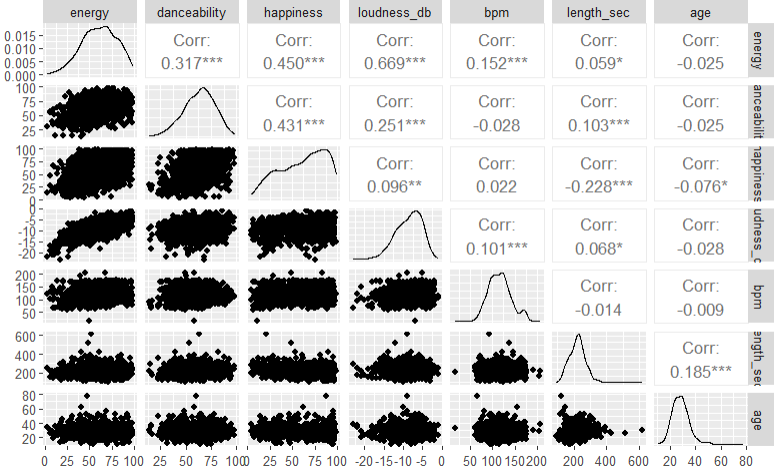
\includegraphics[width=0.6\textwidth]{scatterplots_numeric.png}
\caption{Scatterplot Matrix for Numeric Predictors}
\end{figure}

\noindent In Figure 1, the numeric predictors reveal several moderate correlations among song characteristics. 
\noindent In particular, energy has a positive correlation with happiness and loudness, and danceability shows a mild association with happiness. 
\noindent Predictors such as BPM, song length, and age exhibit relatively weak relationships with the others.
\noindent These observations suggest that some song characteristics may capture similar musical attributes and thus, potential multicollinearity when performing linear regression.

Next, we observe the individual relationships of the categorical predictors: race, gender, and genre. 

\begin{figure}[H]
    \centering
    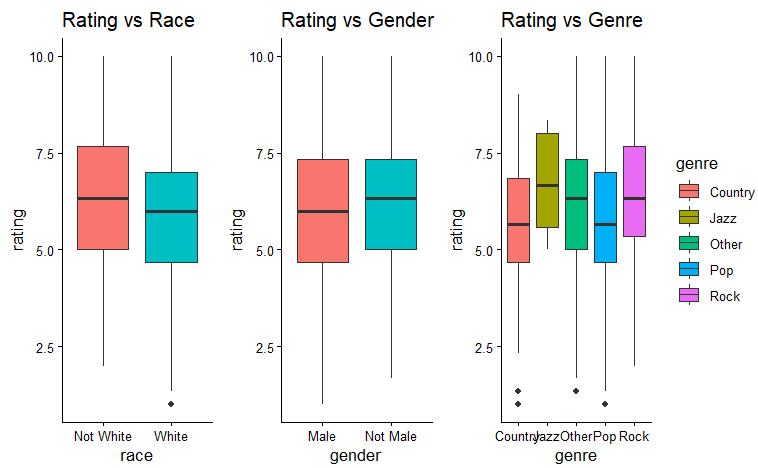
\includegraphics[width=0.6\linewidth]{Boxplots of Categorical Predictors.png}
    \caption{Boxplots of Categorical Predictors}
\end{figure}

\noindent Figure 2 shows that song ratings are fairly similar across race and gender groups. 
\noindent However, some variation appears across genres, with Jazz and Rock tending to have slightly higher median ratings compared to Pop and Country.

\begin{figure}[H]
    \centering
    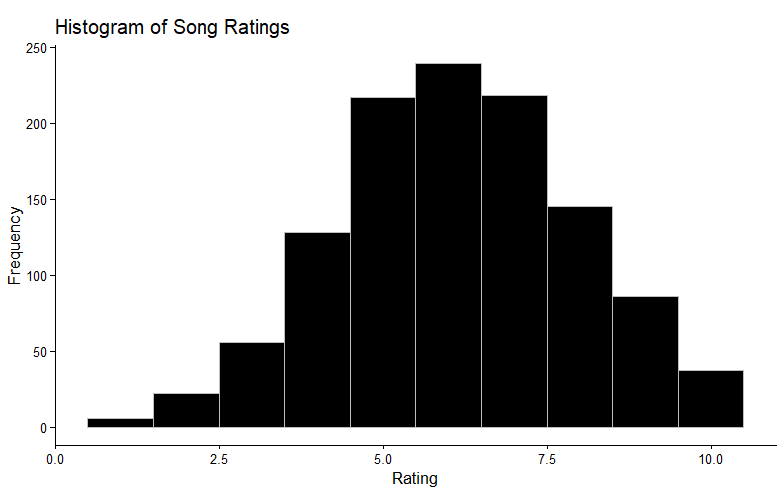
\includegraphics[width=0.5\linewidth]{Histogram.png}
    \caption{Histogram of Song Ratings}
\end{figure}

\noindent Although the overall rating variable is technically discrete, its distribution is approximately symmetric and unimodal. 
\noindent The variable only takes on 30 possible values, making it relatively fine-grained compared to discrete outcomes such as binary variables. 
\noindent Therefore, it is reasonable to treat the response as continuous for linear regression, and no transformation is needed.

\noindent Genre is a main topic of interest as it is one of the most common ways people distingush songs. 

\begin{figure}[H]
    \centering
    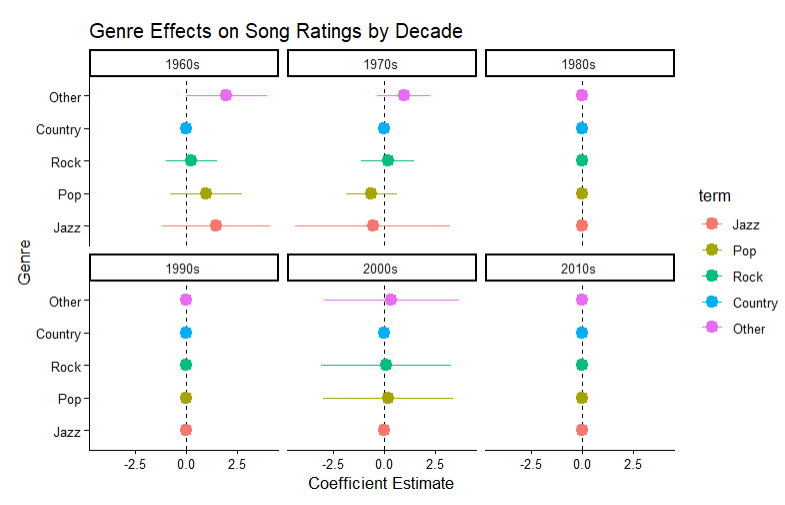
\includegraphics[width=0.65\linewidth]{Genre Coeff Plot.png}
    \caption{Coefficient Esimates Over Time by Genre}
\end{figure}

\noindent Although the coefficient estimates in Figure 4 suggest that genre is consistently an insignificant predictor of ratings, 
\noindent we continue exploring this relationship to determine whether particular genres have a correlation to rating in the dataset. 

\noindent Overall, the exploratory analysis revealed potential multicollinearity among numeric predictors such as energy, happiness, loudness and danceability. 
\noindent On the other hand, BPM, song length, and age showed relatively weak associations with the remaining predictors. 
\noindent The boxplots displayed similar rating distributions across race and gender, with some variation across genres. 
\noindent As a result, the data were divided into decades to better understand how these predictors influence song ratings across different eras.

{\scriptsize First author: Lauren}
% -------------------------------------------------------------------
\section{Methodology and Model Building}
% -------------------------------------------------------------------

\textbf{\underline{Model Fitting Procedure}}

\begin{enumerate}
  \item Fit a main effects and interaction effects model to predict the decade's overall song ratings.
  \item Determine whether the interaction effects model includes substantial predictors that were not
  included in our main effects model by running an anova test at a signficance
  level of 0.1.
  \item If the p-value is significant, run a backwards step procedure (based on AIC) on the interaction effects model. Otherwise, run the backward step
  procedure on the main effects model.
  \item Repeat the previous steps for each decade to acquire the optimized models.
\end{enumerate}

\textbf{\underline{1960s Model}}
\begin{equation}
\begin{aligned}
    Y_i = \beta_0 & + \beta_1 X_{i1} + \beta_2 X_{i2} + \beta_3 X_{i3} + \beta_4 X_{i4} + \beta_5 X_{i5} \\
                  & + \beta_6 X_{i6} + \beta_7 X_{i7} + \beta_8 X_{i8} + \beta_9 X_{i9} + \beta_{10} X_{i10} + \beta_{11} X_{i13} \\
                  & + \beta_{12} (X_{i3}X_{i4}) + \beta_{13} (X_{i3}X_{i7}) + \beta_{14} (X_{i3}X_{i6}) \\
                  & + \beta_{15} (X_{i3}X_{i8}) + \beta_{16} (X_{i3}X_{i9}) + \beta_{17} (X_{i2}X_{i9}) \\
                  & + \beta_{18} (X_{i2}X_{i10}) + \epsilon_i
\end{aligned}
\label{eq:60s_model}
\end{equation}

\textbf{\underline{1970s Model}}
\begin{equation}
\begin{aligned}
    Y_i = \beta_0 & + \beta_1 X_{i1} + \beta_2 X_{i3} + \beta_3 X_{i4} + \beta_4 X_{i5} \\
                  & + \beta_5 X_{i6} + \beta_6 X_{i7} + \beta_{7} X_{i13} + \epsilon_i
\end{aligned}
\label{eq:70s_model}
\end{equation}

\textbf{\underline{1980s Model}}
\begin{equation}
\begin{aligned}
    Y_i = \beta_0 & + \beta_1 X_{i8} + \beta_2 X_{i9} + \beta_3 X_{i10} + \epsilon_i
\end{aligned}
\label{eq:80s_model}
\end{equation}

\textbf{\underline{1990s Model}}
\begin{equation}
\begin{aligned}
    Y_i = \beta_0 & + \beta_1 X_{i2} + \beta_2 X_{i3} + \beta_3 X_{i8} + \beta_4 X_{i10} + \beta_{5} X_{i11} + \epsilon_i
\end{aligned}
\label{eq:90s_model}
\end{equation}

\textbf{\underline{2000s Model}}
\begin{equation}
\begin{aligned}
    Y_i = \beta_0 & + \beta_1 X_{i1} + \beta_2 X_{i2} + \beta_3 X_{i3} + \beta_4 X_{i5} \\
                  & + \beta_5 X_{i6} + \beta_6 X_{i7} + \beta_7 X_{i8} + \beta_8 X_{i9} + \beta_{9} X_{i10} + \beta_{10} X_{i12}\\
                  & + \beta_{11} X_{i13} + \beta_{12} (X_{i1}X_{i9}) + \beta_{13} (X_{i3}X_{i7})\\
                  & + \beta_{14} (X_{i3}X_{i9}) + \beta_{15} (X_{i3}X_{i10}) + \beta_{16} (X_{i3}X_{i12}) \\
                  & + \beta_{17} (X_{i3}X_{i13}) + \beta_{18} (X_{i2}X_{i9}) + \beta_{19} (X_{i2}X_{i10}) \\
                  & + \beta_{20} (X_{i2}X_{i12}) + \epsilon_i
\end{aligned}
\label{eq:2000s_model}
\end{equation}

\textbf{\underline{2010s Model}}
\begin{equation}
\begin{aligned}
    Y_i = \beta_0 & + \beta_1 X_{i2} + \beta_2 X_{i8} + \beta_3 X_{i10} + \beta_4 X_{i13} + \epsilon_i
\end{aligned}
\label{eq:2010s_model}
\end{equation}

{\scriptsize First author: Krish}

% -------------------------------------------------------------------
\section{Results and Diagnostics}
% -------------------------------------------------------------------

\begin{figure}[H]
    \centering
    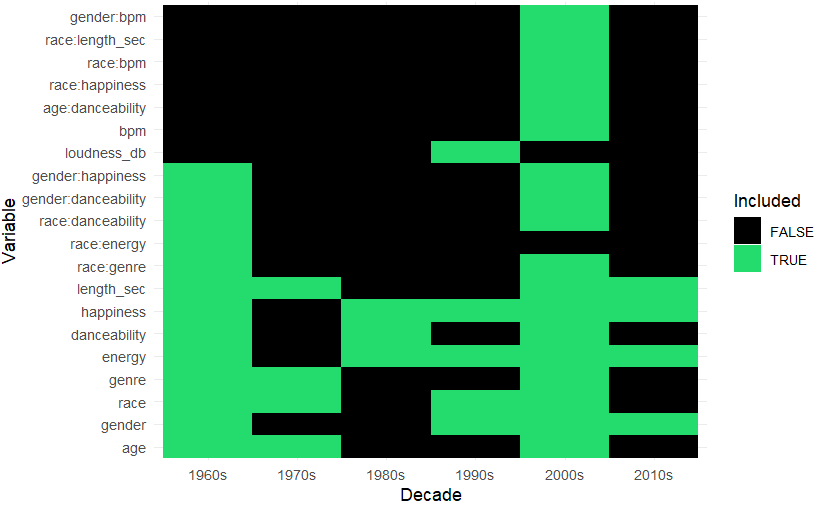
\includegraphics[width=0.5\linewidth]{Presence Matrix Plot.png}
    \caption{Presence Matrix Table}
\end{figure}

\noindent Figure 5 visualizes the inclusion of predictors from each optimized model. The most optimal predictors were
\noindent energy and happiness, occurring in five out of the six decades. The least optimal predictors were 
\noindent race:energy, loudness\_db, bpm, age:danceability, race:happiness, race:bpm, race:length\_sec, gender:bpm.
\noindent In other words, loudness\_db, bpm, and a few interaction terms were predictors for only one decade's optimized model.

\noindent Additionally, the table provides insight into the structure of the models and the inconsistency of variable selection across decades.
\noindent Clearly, the 1960s and 2000s require many predictors, while the other decades rely on a few. 

{\scriptsize First author: Lauren}

\subsection{Proposed Model}

\begin{table}[H]
\centering
\resizebox{0.2\textwidth}{!}{% Scale to 80% of text width
\begin{tabular}{lr}
\toprule
\textbf{Decade} & \textbf{Adjusted $R^2$} \\
\midrule
\rowcolor{yellow}
1960s & 0.245 \\
1970s & 0.201 \\
1980s & 0.010 \\
1990s & 0.215 \\
2000s & 0.220 \\
2010s & 0.064 \\
\bottomrule
\end{tabular}
}
\caption{Adjusted $R^2$ for Each Optimized Model Per Decade}
\end{table}

{\scriptsize First author: Kian}

The adjusted $R^2$ values vary across decades, indicating that predictive power changes over time. 
Nonetheless, we chose the model that explains the greatest proportion of variability in song ratings, while still penalizing model complexity (highest adjusted $R^2$).
The linear model predicting overall song ratings in the 60s performed the best.

\begin{equation}
\begin{aligned}
    Y_i = \beta_0 & + \beta_1 X_{i1} + \beta_2 X_{i2} + \beta_3 X_{i3} + \beta_4 X_{i4} + \beta_5 X_{i5} \\
                  & + \beta_6 X_{i6} + \beta_7 X_{i7} + \beta_8 X_{i8} + \beta_9 X_{i9} + \beta_{10} X_{i10} + \beta_{11} X_{i13} \\
                  & + \beta_{12} (X_{i3}X_{i4}) + \beta_{13} (X_{i3}X_{i7}) + \beta_{14} (X_{i3}X_{i6}) \\
                  & + \beta_{15} (X_{i3}X_{i8}) + \beta_{16} (X_{i3}X_{i9}) + \beta_{17} (X_{i2}X_{i9}) \\
                  & + \beta_{18} (X_{i2}X_{i10}) + \epsilon_i \qquad \text{where } \epsilon_i \overset{iid}{\sim} \mathcal{N}(0, \sigma^2)
\end{aligned}
\end{equation}

{\scriptsize First author: Krish}

\subsection{Model Summary}
Since the 1960s model had the highest adjusted $R^2$ value, we will use it as our final model.

\begin{figure}[H]
\centering
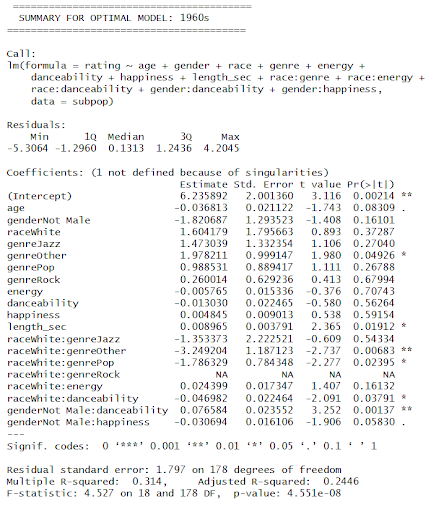
\includegraphics[width=0.45\textwidth]{1960s_Model.png}
\caption{Summary of 1960s Optimized Model}
\end{figure}

{\scriptsize First author: Kian}

\subsection{Model Diagnostics}

\begin{figure}[H]
\centering
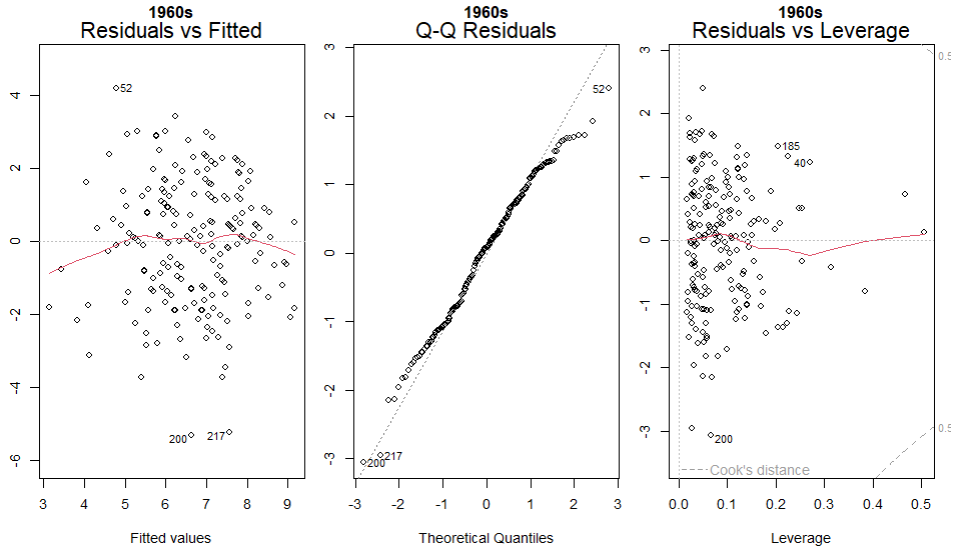
\includegraphics[width=0.6\textwidth]{1960s_all_plots.png}
\caption{TA, QQ, and Residual vs Leverage Plots for the 1960s Model}
\end{figure}

In the TA plot, the residuals are mostly centered around 0, supporting the zero mean assumption. 
They also appear randomly scattered, indicating homoscedasticity. With the QQ plot, we noticed that the tails are somewhat short-tailed on both ends. 
Because of this, we violate the normality assumption. However, we deemed transformations unnecessary since the short tails are without skew.
The residuals vs. leverage plot shows that all of our observations have a Cook's distance of under 0.5, meaning that the outliers are not influential enough for concern.

{\scriptsize First author: Kian}

% -------------------------------------------------------------------
\section{Discussion and Conclusion}
% -------------------------------------------------------------------

\noindent The 1960s model was selected as the proposed model because it demonstrated the best adjusted $R^2$. 
\noindent Each coefficient represents the expected change in song rating associated with a one-unit increase in a predictor, holding other variables constant. 
\noindent Among the predictors, song length shows a positive relationship with rating, leading us to believe that longer songs tend to receive slightly higher ratings on average. 
\noindent Some genre effects also appear, with the coefficient for the “Other” genre having a modest difference relative to the baseline genre. 
\noindent Several interaction terms are present, suggesting that the effects of certain song characteristics vary depending on artist attributes 
\noindent such as race or gender. Overall, both song and artist characteristics contribute to variation in song ratings.

\noindent One of the limitations is the low adjusted $R^2$, even with a large number of predictors. Splitting into decades resulted in a smaller dataset for each decade. 
\noindent Thus, more data would be better for preventing NAs. In addition, the model most likely would not generalize well to other songs since it is based on number one songs in the 1960s. 

{\scriptsize First author: Lauren}
\vspace{-0.3cm}
\begin{thebibliography}{9}

\bibitem{dataset}
Chris Dalla Riva.
\textit{Billboard Hot 100 Number Ones}.
\url{https://github.com/rfordatascience/tidytuesday/tree/main/data/2025/2025-08-26}

\end{thebibliography}


% -------------------------------------------------------------------
\newpage
\appendix
\section{Appendix: Code}
% -------------------------------------------------------------------

\subsection{Cleaning Data}
\begin{verbatim}
orig_data <- read.csv("billboard.csv")

cleaned_data <- data.frame(artist = orig_data$artist, rating = orig_data$overall_rating, 
  age=orig_data$front_person_age)

cleaned_data$gender <- ifelse(orig_data$artist_male == 1, "Male", "Not Male")

cleaned_data$race <- ifelse(orig_data$artist_white == 1, "White", "Not White")

cleaned_data$genre <- ifelse(is.na(orig_data$cdr_genre), "Genre Not Specified", 
    orig_data$cdr_genre)

cleaned_data$genre <- ifelse(grepl("Pop", orig_data$cdr_genre), "Pop", 
                      ifelse(grepl("Country", orig_data$cdr_genre), "Country",
                      ifelse(grepl("Hip-Hop", orig_data$cdr_genre), "Hip-Hop",
                      ifelse(grepl("Rock", orig_data$cdr_genre), "Rock",
                      ifelse(grepl("Jazz", orig_data$cdr_genre), "Jazz", "Other")))))

cleaned_data <- cbind(cleaned_data, bpm=orig_data$bpm, energy=orig_data$energy, 
                danceability = orig_data$danceability, happiness = orig_data$happiness, 
                loudness_db = orig_data$loudness_d_b, 
                length_sec = orig_data$length_sec)


cleaned_data$year <- as.numeric(substr(orig_data$date, 1, 
                    unlist(gregexpr("-", orig_data$date))[1] - 1))

cleaned_data <- cleaned_data[rowSums(is.na(cleaned_data)) == 0 , ]
\end{verbatim}

\subsection{Finding Optimized Models}
\begin{verbatim}
model_results <- list()


for(i in seq(1960, 2030, 10)){
  decade_label <- paste0(i - 10, "s")

  subpop <- cleaned_data[cleaned_data$year >= i - 10 & 
                          cleaned_data$year < i, ]
  
  # --- SAFETY CHECK 1: Ensure enough rows exist ---
  # If you have < 50 rows, the interaction model will likely fail.
  if(nrow(subpop) < 50) {
    message(paste("Skipping", decade_label, "- Not enough data points."))
    next
  }
  
  factor_counts <- sapply(subpop[, c("genre", "gender", "race")], 
                  function(x) length(unique(na.omit(x))))
  
  if(any(factor_counts < 2)) {
    message(paste("Skipping", decade_label, "due to single-level factor:", 
                  names(factor_counts)[factor_counts < 2]))
    next
  }
  
  first_model <- lm(data = subpop, rating ~ age + race + gender + genre + energy 
                  + danceability + happiness + bpm + loudness_db + length_sec)

  second_model <- lm(data = subpop, rating ~ age + gender + race + age*genre 
                + age*energy + age*danceability + age*happiness + age*bpm 
                + age*loudness_db + age*length_sec + race*genre + race*energy 
                + race*danceability + race*happiness + race*bpm + race*loudness_db 
                + race*length_sec + gender*genre + gender*energy + gender*danceability 
                + gender*happiness + gender*bpm +gender*loudness_db + gender*length_sec)
  

  if(anova(first_model, second_model)$"Pr(>F)"[2] <= 0.1){
     optimal_model <<- step(second_model, direction="backward")
  } else {
      optimal_model <<- step(first_model, direction="backward")
  }
  
  
  model_results[[decade_label]] <- list(
    "first"   = first_model,
    "second"  = second_model,
    "optimal" = optimal_model
  )
  
  print(decade_label)
  summary(first_model)
  summary(second_model)
  summary(optimal_model)
}
\end{verbatim}

\subsection{Model Interpretations and Assumptions}
\begin{verbatim}

model_60s <- model_results[["1960s"]]$optimal
model_70s <- model_results[["1970s"]]$optimal
model_80s <- model_results[["1980s"]]$optimal
model_90s <- model_results[["1990s"]]$optimal
model_2000s <- model_results[["2000s"]]$optimal
model_2010s <- model_results[["2010s"]]$optimal

summary(model_60s)
summary(model_70s)
summary(model_80s)
summary(model_90s)
summary(model_2000s)
summary(model_2010s)

# TA, QQ, and Leverage vs. Residuals Plots

par(mfrow = c(1,3), mar = c(5, 2, 4, 1))

plot(model_60s, which = c(1, 2, 5), main = "1960s")

\end{verbatim}

\subsection{Predictor and Genre C.I Analysis}
\begin{verbatim}
library("GGally")

# Scatterplot Matrix
ggpairs(data = cleaned_data[,c("energy", "danceability", "happiness", "loudness_db", "bpm", "length_sec", "age")])

# Boxplots
plot_race <- ggplot(cleaned_data, aes(x = race, y = rating, fill = race)) +
  geom_boxplot() +
  theme_classic() +
  ggtitle("Rating vs Race") + 
  guides(fill = "none")

plot_gender <- ggplot(cleaned_data, aes(x = gender, y = rating, fill = gender)) +
  geom_boxplot() +
  theme_classic() +
  ggtitle("Rating vs Gender") + 
  guides(fill = "none")

plot_genre <- ggplot(cleaned_data, aes(x = genre, y = rating, fill = genre)) +
  geom_boxplot() +
  theme_classic() +
  ggtitle("Rating vs Genre")

plot_race + plot_gender + plot_genre 

# Rating Histogram
ggplot(cleaned_data, aes(x = rating)) +
  geom_histogram(
    binwidth = 1,
    boundary = 0.5, 
    fill = "black",  
    color = "grey",
    linewidth = 0.3
  ) +
  labs(
    title = "Histogram of Song Ratings",
    x = "Rating",
    y = "Frequency"
  ) +
  theme_classic()
  
# Genre Confidence Intervals Per Decade
  
library(broom)
coef_1960s <- tidy(model_60s, conf.int = TRUE) %>% mutate(decade = "1960s")
coef_1970s <- tidy(model_70s, conf.int = TRUE) %>% mutate(decade = "1970s")
coef_1980s <- tidy(model_80s, conf.int = TRUE) %>% mutate(decade = "1980s")
coef_1990s <- tidy(model_90s, conf.int = TRUE) %>% mutate(decade = "1990s")
coef_2000s <- tidy(model_2000s, conf.int = TRUE) %>% mutate(decade = "2000s")
coef_2010s <- tidy(model_2010s, conf.int = TRUE) %>% mutate(decade = "2010s")


#Appending Data not Represented
#1960s
coef_1960s <- rbind(coef_1960s, list("genreCountry", 0, 0, 0, 0, 0, 0, "1960s"))

#1970s
coef_1970s <- rbind(coef_1970s, list("genreCountry", 0, 0, 0, 0, 0, 0, "1970s"))

#1980s
coef_1980s <- rbind(coef_1980s, list("genreCountry", 0, 0, 0, 0, 0, 0, "1980s"))
coef_1980s <- rbind(coef_1980s, list("genreOther", 0, 0, 0, 0, 0, 0, "1980s"))
coef_1980s <- rbind(coef_1980s, list("genreJazz", 0, 0, 0, 0, 0, 0, "1980s"))
coef_1980s <- rbind(coef_1980s, list("genreRock", 0, 0, 0, 0, 0, 0, "1980s"))
coef_1980s <- rbind(coef_1980s, list("genrePop", 0, 0, 0, 0, 0, 0, "1980s"))

#1990s
coef_1990s <- rbind(coef_1990s, list("genreCountry", 0, 0, 0, 0, 0, 0, "1990s"))
coef_1990s <- rbind(coef_1990s, list("genreOther", 0, 0, 0, 0, 0, 0, "1990s"))
coef_1990s <- rbind(coef_1990s, list("genreJazz", 0, 0, 0, 0, 0, 0, "1990s"))
coef_1990s <- rbind(coef_1990s, list("genreRock", 0, 0, 0, 0, 0, 0, "1990s"))
coef_1990s <- rbind(coef_1990s, list("genrePop", 0, 0, 0, 0, 0, 0, "1990s"))


#2000s
coef_2000s <- rbind(coef_2000s, list("genreCountry", 0, 0, 0, 0, 0, 0, "2000s"))
coef_2000s <- rbind(coef_2000s, list("genreJazz", 0, 0, 0, 0, 0, 0, "2000s"))

#2010s
coef_2010s <- rbind(coef_2010s, list("genreCountry", 0, 0, 0, 0, 0, 0, "2010s"))
coef_2010s <- rbind(coef_2010s, list("genreOther", 0, 0, 0, 0, 0, 0, "2010s"))
coef_2010s <- rbind(coef_2010s, list("genreJazz", 0, 0, 0, 0, 0, 0, "2010s"))
coef_2010s <- rbind(coef_2010s, list("genreRock", 0, 0, 0, 0, 0, 0, "2010s"))
coef_2010s <- rbind(coef_2010s, list("genrePop", 0, 0, 0, 0, 0, 0, "2010s"))




coef_data <- bind_rows(
  coef_1960s,
  coef_1970s,
  coef_1980s,
  coef_1990s,
  coef_2000s,
  coef_2010s
)

coef_data <- coef_data %>%
  filter(term != "(Intercept)") %>%
  filter(grepl("^genre", term)) %>%
  mutate(term = gsub("^genre", "", term))

coef_data$term <- factor(
  coef_data$term,
  levels = c("Jazz","Pop","Rock","Country","HipHop","Other")
)

ggplot(coef_data, aes(x = estimate, y = term, color = term)) +
  geom_vline(xintercept = 0, linetype = "dashed") +
  geom_pointrange(aes(xmin = conf.low, xmax = conf.high), size = 0.8) +
  facet_wrap(~ decade) +
  theme_classic() +
  labs(
    title = "Genre Effects on Song Ratings by Decade",
    x = "Coefficient Estimate",
    y = "Genre"
  )
\end{verbatim}



\subsection{Adjusted $R^2$ Comparison}
\begin{verbatim}
summary(model_60s)$adj.r.squared

summary(model_70s)$adj.r.squared

summary(model_80s)$adj.r.squared

summary(model_90s)$adj.r.squared

summary(model_2000s)$adj.r.squared

summary(model_2010s)$adj.r.squared

library(ggplot2)

df <- data.frame(
  Decade = factor(c("1960s","1970s","1980s","1990s","2000s","2010s"),
                  levels = c("2010s","2000s","1990s","1980s","1970s","1960s")),
  Adj_R2 = c(0.244647, 0.2013403, 0.009698796, 0.2152039, 0.2197517, 0.06362834)
)

ggplot(df, aes(x = Decade, y = Adj_R2)) +
  geom_col(fill = "#23DC6D") +
  geom_text(aes(label = round(Adj_R2,3)), hjust = -0.1, size = 4) +
  coord_flip() +
  ylim(0, 0.3) +
  labs(
    title = "Adjusted R2 of Song Rating Models by Decade",
    x = "Decade",
    y = "Adjusted R2"
  ) +
  theme_minimal(base_size = 14)
  
  
\end{verbatim}

\subsection{Presence Matrix}
\begin{verbatim}
vars_by_decade <- lapply(model_results, function(x) {
  attr(terms(x$optimal), "term.labels")
})

all_vars <- unique(unlist(vars_by_decade))

presence_matrix <- sapply(vars_by_decade, function(vars) {
  all_vars %in% vars
})

rownames(presence_matrix) <- all_vars
presence_matrix

presence_df <- as.data.frame(as.table(presence_matrix))

ggplot(presence_df, aes(x = Var2, y = Var1, fill = Freq)) +
  geom_tile() +
  scale_fill_manual(values = c("black","#23DC6D")) +
  labs(x = "Decade", y = "Variable", fill = "Included") +
  theme_minimal()

true_counts <- rowSums(presence_matrix)
true_counts

rownames(presence_matrix)[true_counts == max(true_counts)]

false_counts <- rowSums(!presence_matrix)
false_counts

rownames(presence_matrix)[false_counts == max(false_counts)]

summary_table <- data.frame(
  TRUE_count = rowSums(presence_matrix),
  FALSE_count = rowSums(!presence_matrix)
)

summary_table[order(-summary_table$TRUE_count), ]
\end{verbatim}

\end{document}